%!TEX root = ../main.tex
% Chapter 9 — Numerical Solution of ODEs

\chapter{Numerical Solution of Ordinary Differential Equations}
\label{ch:ode}


\section{Introduction}

Many phenomena in physics, biology, and engineering are modeled by ordinary differential equations (ODEs) that cannot be solved analytically. This chapter introduces the fundamental numerical methods for initial value problems.

%==============================================================================
\section{The Cauchy Problem}
%==============================================================================

\begin{definition}[Initial value problem / Cauchy problem]
\label{def:cauchy}
\index{Cauchy problem}
\index{initial value problem}
Given $f: [t_0, T] \times \R^d \to \R^d$, find $y: [t_0, T] \to \R^d$ such that
\[
    \begin{cases}
        y'(t) = f(t, y(t)), & t \in [t_0, T], \\
        y(t_0) = y_0.
    \end{cases}
\]
\end{definition}

\begin{theorem}[Picard--Lindel\"of]
\label{thm:picard}
\index{Picard--Lindel\"of theorem}
If $f$ is continuous in $t$ and Lipschitz continuous in $y$ with Lipschitz constant $L$:
\[
    \|f(t,y_1) - f(t,y_2)\| \leq L\,\|y_1 - y_2\| \quad \forall\, t \in [t_0, T],\; y_1, y_2 \in \R^d,
\]
then the Cauchy problem has a unique solution on $[t_0, T]$.
\end{theorem}

We discretize $[t_0, T]$ with a uniform grid: $t_n = t_0 + nh$, $h = (T-t_0)/N$, and seek approximations $y_n \approx y(t_n)$.

%==============================================================================
\section{Euler's Methods}
%==============================================================================

\subsection{Explicit (forward) Euler method}

\begin{definition}[Explicit Euler method]
\label{def:euler-explicit}
\index{Euler method!explicit}
\[
    y_{n+1} = y_n + h\,f(t_n, y_n), \qquad n = 0, 1, \ldots, N-1.
\]
\end{definition}

\begin{algorithm}[H]
\caption{Explicit Euler method}
\label{alg:euler-explicit}
\KwInput{$f$, $t_0$, $T$, $y_0$, $N$ (number of steps)}
\KwOutput{Arrays $t[0:N]$, $y[0:N]$}
$h \gets (T - t_0) / N$\;
$t[0] \gets t_0$\;
$y[0] \gets y_0$\;
\For{$n = 0, 1, \ldots, N-1$}{
    $y[n+1] \gets y[n] + h \cdot f(t[n], y[n])$\;
    $t[n+1] \gets t[n] + h$\;
}
\Return{$t$, $y$}\;
\end{algorithm}

\begin{theorem}[Global error of explicit Euler]
\label{thm:euler-error}
\index{Euler method!error}
If $f$ is Lipschitz in $y$ with constant $L$ and $y \in C^2([t_0,T])$, then
\[
    \max_{0 \leq n \leq N} \|y(t_n) - y_n\| \leq \frac{hM}{2L}\left(e^{L(T-t_0)} - 1\right),
\]
where $M = \max_{t \in [t_0,T]} \|y''(t)\|$. The method is of \textbf{order 1}: the global error is $\BigO(h)$.
\end{theorem}

\begin{proof}
\textbf{Local truncation error.} Taylor-expanding:
\[
    y(t_{n+1}) = y(t_n) + h\,y'(t_n) + \frac{h^2}{2}\,y''(\xi_n) = y(t_n) + h\,f(t_n, y(t_n)) + \frac{h^2}{2}\,y''(\xi_n).
\]
The local truncation error is $\tau_n = \frac{h}{2}\,y''(\xi_n)$, so $|\tau_n| \leq \frac{hM}{2}$.

\textbf{Global error.} Let $e_n = y(t_n) - y_n$. Then:
\begin{align*}
    e_{n+1} &= y(t_{n+1}) - y_{n+1} \\
    &= \bigl[y(t_n) + h\,f(t_n, y(t_n)) + h\tau_n\bigr] - \bigl[y_n + h\,f(t_n, y_n)\bigr] \\
    &= e_n + h\bigl[f(t_n, y(t_n)) - f(t_n, y_n)\bigr] + h\tau_n.
\end{align*}
Using the Lipschitz condition:
\[
    \|e_{n+1}\| \leq (1 + hL)\|e_n\| + h\,\frac{hM}{2}.
\]
Setting $\delta = \frac{hM}{2}$ and iterating with $e_0 = 0$:
\[
    \|e_n\| \leq \frac{\delta}{hL}\bigl[(1+hL)^n - 1\bigr] \leq \frac{hM}{2L}\bigl[e^{nhL} - 1\bigr] \leq \frac{hM}{2L}\bigl[e^{L(T-t_0)} - 1\bigr],
\]
using the inequality $(1+hL)^n \leq e^{nhL}$.
\end{proof}

\subsection{Implicit (backward) Euler method}

\begin{definition}[Implicit Euler method]
\label{def:euler-implicit}
\index{Euler method!implicit}
\[
    y_{n+1} = y_n + h\,f(t_{n+1}, y_{n+1}), \qquad n = 0, 1, \ldots, N-1.
\]
This is an implicit equation for $y_{n+1}$ and generally requires solving a nonlinear system at each step (e.g., by Newton's method).
\end{definition}

\begin{definition}[A-stability]
\label{def:A-stability}
\index{A-stability}
A numerical method is \textbf{A-stable} if its stability region contains the entire left half of the complex plane: $\{z \in \C : \operatorname{Re}(z) \leq 0\} \subset \mathcal{S}$.
\end{definition}

\begin{theorem}
\label{thm:implicit-euler-Astable}
The implicit Euler method is A-stable.
\end{theorem}

\begin{proof}
For the test equation $y' = \lambda y$ ($\lambda \in \C$), the implicit Euler gives:
\[
    y_{n+1} = y_n + h\lambda\,y_{n+1} \implies y_{n+1} = \frac{y_n}{1 - h\lambda}.
\]
The amplification factor is $R(z) = \frac{1}{1-z}$ where $z = h\lambda$. Stability requires $|R(z)| \leq 1$, i.e., $|1-z| \geq 1$. For $z = x + iy$ with $x \leq 0$: $|1-z|^2 = (1-x)^2 + y^2 \geq 1$ since $1-x \geq 1$. Thus $|R(z)| \leq 1$ for all $\operatorname{Re}(z) \leq 0$.
\end{proof}

%==============================================================================
\section{Runge--Kutta Methods}
%==============================================================================

\begin{definition}[General $s$-stage Runge--Kutta method]
\label{def:runge-kutta}
\index{Runge--Kutta method}
An $s$-stage Runge--Kutta method is defined by
\begin{align*}
    k_i &= f\!\left(t_n + c_i h,\; y_n + h\sum_{j=1}^{s} a_{ij}\,k_j\right), \qquad i = 1, \ldots, s, \\
    y_{n+1} &= y_n + h\sum_{i=1}^{s} b_i\,k_i.
\end{align*}
The method is \textbf{explicit} if $a_{ij} = 0$ for $j \geq i$.
\end{definition}

\begin{definition}[Butcher tableau]
\label{def:butcher}
\index{Butcher tableau}
A Runge--Kutta method is compactly represented by its \textbf{Butcher tableau}:
\[
\renewcommand{\arraystretch}{1.2}
\begin{array}{c|c}
    \mathbf{c} & \mathbf{A} \\
    \hline
    & \mathbf{b}^\top
\end{array}
\qquad = \qquad
\begin{array}{c|cccc}
    c_1 & a_{11} & a_{12} & \cdots & a_{1s} \\
    c_2 & a_{21} & a_{22} & \cdots & a_{2s} \\
    \vdots & \vdots & \vdots & \ddots & \vdots \\
    c_s & a_{s1} & a_{s2} & \cdots & a_{ss} \\
    \hline
    & b_1 & b_2 & \cdots & b_s
\end{array}
\]
with the consistency condition $c_i = \sum_{j=1}^{s} a_{ij}$.
\end{definition}

\subsection{Classical fourth-order Runge--Kutta (RK4)}

\begin{definition}[RK4]
\label{def:rk4}
\index{Runge--Kutta method!RK4}
The classical RK4 method:
\begin{align*}
    k_1 &= f(t_n, y_n), \\
    k_2 &= f(t_n + h/2, \; y_n + (h/2)\,k_1), \\
    k_3 &= f(t_n + h/2, \; y_n + (h/2)\,k_2), \\
    k_4 &= f(t_n + h, \; y_n + h\,k_3), \\
    y_{n+1} &= y_n + \frac{h}{6}(k_1 + 2k_2 + 2k_3 + k_4).
\end{align*}
Butcher tableau:
\[
\begin{array}{c|cccc}
    0   &     &     &     &   \\
    1/2 & 1/2 &     &     &   \\
    1/2 & 0   & 1/2 &     &   \\
    1   & 0   & 0   & 1   &   \\
    \hline
        & 1/6 & 1/3 & 1/3 & 1/6
\end{array}
\]
\end{definition}

\begin{theorem}[Order of RK4]
\label{thm:rk4-order}
The classical RK4 method has \textbf{order 4}: the global error is $\BigO(h^4)$ and the local truncation error is $\BigO(h^5)$.
\end{theorem}

\begin{remark}
For explicit Runge--Kutta methods:
\begin{center}
\begin{tabular}{lcc}
    \toprule
    \textbf{Method} & \textbf{Stages} & \textbf{Order} \\
    \midrule
    Euler       & 1 & 1 \\
    Heun (RK2)  & 2 & 2 \\
    Kutta (RK3) & 3 & 3 \\
    Classic RK4 & 4 & 4 \\
    \bottomrule
\end{tabular}
\end{center}
For $s \geq 5$ stages, the maximum achievable order is less than $s$ (Butcher barrier).
\end{remark}

%==============================================================================
\section{Stability Analysis}
%==============================================================================

\begin{definition}[Test equation]
\label{def:test-equation}
\index{test equation}
The Dahlquist test equation is $y' = \lambda y$, $y(0) = 1$, with $\lambda \in \C$. Any one-step method applied to this equation produces
\[
    y_{n+1} = R(z)\,y_n, \qquad z = h\lambda,
\]
where $R(z)$ is the \textbf{amplification factor} (or stability function).
\end{definition}

\begin{definition}[Stability region]
\label{def:stability-region}
\index{stability region}
The \textbf{stability region} of a method is
\[
    \mathcal{S} = \{z \in \C : |R(z)| \leq 1\}.
\]
For the exact solution $|e^{z}| \leq 1$ when $\operatorname{Re}(z) \leq 0$, so a method is A-stable if $\mathcal{S} \supseteq \{z : \operatorname{Re}(z) \leq 0\}$.
\end{definition}

\begin{proposition}[Amplification factors]
\label{prop:amplification}
\index{amplification factor}
\begin{center}
\begin{tabular}{ll}
    \toprule
    \textbf{Method} & $R(z)$ \\
    \midrule
    Explicit Euler  & $1 + z$ \\
    Implicit Euler  & $\dfrac{1}{1-z}$ \\
    Trapezoidal (Crank--Nicolson) & $\dfrac{1+z/2}{1-z/2}$ \\
    RK4             & $1 + z + \dfrac{z^2}{2} + \dfrac{z^3}{6} + \dfrac{z^4}{24}$ \\
    \bottomrule
\end{tabular}
\end{center}
\end{proposition}

\begin{remark}
The explicit Euler stability region is the disk $|1+z| \leq 1$, centered at $(-1,0)$ with radius $1$. For the explicit Euler applied to $y' = \lambda y$ with $\lambda < 0$, stability requires $0 < h < 2/|\lambda|$.
\end{remark}

\subsection{Stability region plots}

\begin{figure}[htbp]
\centering
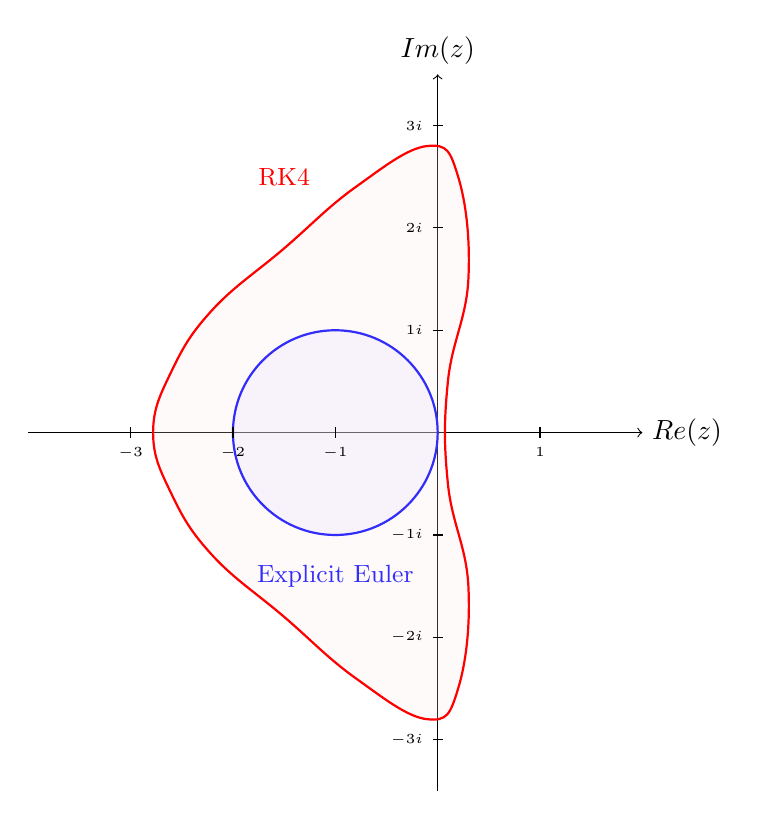
\begin{tikzpicture}[scale=1.3]
    % Axes
    \draw[->] (-4,0) -- (2,0) node[right] {$\operatorname{Re}(z)$};
    \draw[->] (0,-3.5) -- (0,3.5) node[above] {$\operatorname{Im}(z)$};

    % Explicit Euler: |1+z| <= 1, circle centered at (-1,0) radius 1
    \draw[blue, thick, fill=blue!10, fill opacity=0.3] (-1,0) circle (1);
    \node[blue] at (-1,-1.4) {\small Explicit Euler};

    % RK4 stability region (approximate boundary)
    \draw[red, thick, fill=red!10, fill opacity=0.2]
        plot[smooth cycle, tension=0.7] coordinates {
            (-2.78,0) (-2.6,0.6) (-2.2,1.2) (-1.5,1.8)
            (-0.8,2.4) (-0.1,2.8) (0.2,2.5) (0.3,1.5)
            (0.1,0.5) (0.1,-0.5) (0.3,-1.5) (0.2,-2.5)
            (-0.1,-2.8) (-0.8,-2.4) (-1.5,-1.8) (-2.2,-1.2)
            (-2.6,-0.6)
        };
    \node[red] at (-1.5,2.5) {\small RK4};

    % Grid
    \foreach \x in {-3,-2,-1,1}
        \draw (\x,0.05) -- (\x,-0.05) node[below] {\tiny $\x$};
    \foreach \y in {-3,-2,-1,1,2,3}
        \draw (0.05,\y) -- (-0.05,\y) node[left] {\tiny $\y i$};
\end{tikzpicture}
\caption{Stability regions of explicit Euler (blue) and RK4 (red) in the complex $z = h\lambda$ plane.}
\label{fig:stability-regions}
\end{figure}

%==============================================================================
\section{Convergence Study: $y' = -y$}
%==============================================================================

\begin{example}[Convergence table]
\label{ex:ode-convergence}
We solve $y' = -y$, $y(0) = 1$ on $[0,1]$ (exact: $y(1) = e^{-1}$):

\begin{center}
\begin{tabular}{r|cc|cc|cc}
    \toprule
    $N$ & $|e_N^{\text{Euler}}|$ & order & $|e_N^{\text{Heun}}|$ & order & $|e_N^{\text{RK4}}|$ & order \\
    \midrule
    10   & $1.7\times10^{-2}$ & ---  & $4.1\times10^{-4}$ & ---  & $1.5\times10^{-7}$ & --- \\
    20   & $8.5\times10^{-3}$ & 1.0  & $1.0\times10^{-4}$ & 2.0  & $9.3\times10^{-9}$ & 4.0 \\
    40   & $4.2\times10^{-3}$ & 1.0  & $2.6\times10^{-5}$ & 2.0  & $5.8\times10^{-10}$& 4.0 \\
    80   & $2.1\times10^{-3}$ & 1.0  & $6.4\times10^{-6}$ & 2.0  & $3.6\times10^{-11}$& 4.0 \\
    160  & $1.1\times10^{-3}$ & 1.0  & $1.6\times10^{-6}$ & 2.0  & $2.3\times10^{-12}$& 4.0 \\
    \bottomrule
\end{tabular}
\end{center}
\end{example}

%==============================================================================
\section{Implementations}
%==============================================================================

\begin{codeblock}[title=\textbf{Python --- ODE solvers}]
\begin{minted}{python}
import numpy as np
import matplotlib.pyplot as plt

def euler_explicit(f, t0, T, y0, N):
    """Explicit Euler method."""
    h = (T - t0) / N
    t = np.linspace(t0, T, N + 1)
    y = np.zeros((N + 1, len(np.atleast_1d(y0))))
    y[0] = y0
    for n in range(N):
        y[n+1] = y[n] + h * f(t[n], y[n])
    return t, y

def euler_implicit(f, jac, t0, T, y0, N, tol=1e-12):
    """Implicit Euler method (Newton iteration)."""
    h = (T - t0) / N
    t = np.linspace(t0, T, N + 1)
    d = len(np.atleast_1d(y0))
    y = np.zeros((N + 1, d))
    y[0] = y0
    for n in range(N):
        # Newton iteration: G(u) = u - y[n] - h*f(t[n+1], u) = 0
        u = y[n].copy()  # initial guess
        for _ in range(50):
            G = u - y[n] - h * f(t[n+1], u)
            dG = np.eye(d) - h * jac(t[n+1], u)
            delta = np.linalg.solve(dG, -G)
            u += delta
            if np.linalg.norm(delta) < tol:
                break
        y[n+1] = u
    return t, y

def rk4(f, t0, T, y0, N):
    """Classical RK4 method."""
    h = (T - t0) / N
    t = np.linspace(t0, T, N + 1)
    y = np.zeros((N + 1, len(np.atleast_1d(y0))))
    y[0] = y0
    for n in range(N):
        k1 = f(t[n], y[n])
        k2 = f(t[n] + h/2, y[n] + h/2 * k1)
        k3 = f(t[n] + h/2, y[n] + h/2 * k2)
        k4 = f(t[n] + h, y[n] + h * k3)
        y[n+1] = y[n] + (h/6) * (k1 + 2*k2 + 2*k3 + k4)
    return t, y

# Test: y' = -y, y(0) = 1
f = lambda t, y: -y
y0 = np.array([1.0])
y_exact = lambda t: np.exp(-t)

print(f"{'N':>5} {'Euler':>14} {'order':>6} "
      f"{'RK4':>14} {'order':>6}")
print("-" * 50)
err_e_prev = err_r_prev = None
for N in [10, 20, 40, 80, 160, 320]:
    t_e, y_e = euler_explicit(f, 0, 1, y0, N)
    t_r, y_r = rk4(f, 0, 1, y0, N)
    err_e = abs(y_e[-1, 0] - y_exact(1.0))
    err_r = abs(y_r[-1, 0] - y_exact(1.0))
    ord_e = np.log2(err_e_prev/err_e) if err_e_prev else float('nan')
    ord_r = np.log2(err_r_prev/err_r) if err_r_prev else float('nan')
    print(f"{N:5d} {err_e:14.2e} {ord_e:6.2f} "
          f"{err_r:14.2e} {ord_r:6.2f}")
    err_e_prev, err_r_prev = err_e, err_r
\end{minted}
\end{codeblock}

\begin{codeblock}[title=\textbf{Julia --- ODE solvers}]
\begin{minted}{julia}
function euler_explicit(f, t0, T, y0, N)
    h = (T - t0) / N
    t = range(t0, T, length=N+1)
    d = length(y0)
    y = zeros(d, N+1)
    y[:, 1] = y0
    for n in 1:N
        y[:, n+1] = y[:, n] + h * f(t[n], y[:, n])
    end
    return collect(t), y
end

function rk4(f, t0, T, y0, N)
    h = (T - t0) / N
    t = range(t0, T, length=N+1)
    d = length(y0)
    y = zeros(d, N+1)
    y[:, 1] = y0
    for n in 1:N
        k1 = f(t[n], y[:, n])
        k2 = f(t[n] + h/2, y[:, n] + h/2 * k1)
        k3 = f(t[n] + h/2, y[:, n] + h/2 * k2)
        k4 = f(t[n] + h, y[:, n] + h * k3)
        y[:, n+1] = y[:, n] + (h/6) * (k1 + 2k2 + 2k3 + k4)
    end
    return collect(t), y
end

# Test: y' = -y
f(t, y) = -y
y0 = [1.0]

for N in [10, 20, 40, 80, 160]
    t_e, y_e = euler_explicit(f, 0.0, 1.0, y0, N)
    t_r, y_r = rk4(f, 0.0, 1.0, y0, N)
    err_e = abs(y_e[1, end] - exp(-1.0))
    err_r = abs(y_r[1, end] - exp(-1.0))
    @printf("N = %4d: Euler = %.2e, RK4 = %.2e\n",
            N, err_e, err_r)
end
\end{minted}
\end{codeblock}

%==============================================================================
\section{Exercises}
%==============================================================================

\begin{exercise}[$\star$]
\label{ex:ch9-euler-hand}
Apply the explicit Euler method with $h = 0.25$ to solve $y' = -2y$, $y(0)=1$ on $[0,1]$. Compare with the exact solution $y(t) = e^{-2t}$.
\end{exercise}

\begin{exercise}[$\star$]
\label{ex:ch9-stability-euler}
For the test equation $y' = \lambda y$ with $\lambda = -10$:
\begin{enumerate}
    \item Determine the maximum step size $h$ for which the explicit Euler method is stable.
    \item Show that the implicit Euler method is stable for any $h > 0$.
\end{enumerate}
\end{exercise}

\begin{exercise}[$\star\star$]
\label{ex:ch9-rk2-butcher}
The midpoint method has Butcher tableau:
\[
\begin{array}{c|cc}
    0   &     &   \\
    1/2 & 1/2 &   \\
    \hline
        & 0   & 1
\end{array}
\]
\begin{enumerate}
    \item Write out the method explicitly.
    \item Show it has order 2 by verifying the order conditions.
    \item Determine its stability function $R(z)$ and plot the stability region.
\end{enumerate}
\end{exercise}

\begin{exercise}[$\star\star$]
\label{ex:ch9-convergence-table}
Reproduce the convergence table of Example~\ref{ex:ode-convergence}. Verify numerically the convergence orders of explicit Euler, Heun's method, and RK4.
\end{exercise}

\begin{exercise}[$\star\star$]
\label{ex:ch9-stiff}
Consider the stiff system
\[
    y' = -1000(y - \sin t) + \cos t, \qquad y(0) = 0.
\]
\begin{enumerate}
    \item Solve with explicit Euler for $h = 0.001$ and $h = 0.003$. What happens?
    \item Solve with implicit Euler for $h = 0.01$ and $h = 0.1$.
    \item Explain the results using stability analysis.
\end{enumerate}
\end{exercise}

\begin{exercise}[$\star\star\star$ --- Project: Lorenz system]
\label{ex:ch9-lorenz}
\index{Lorenz system}
The Lorenz system is
\[
    \begin{cases}
        \dot{x} = \sigma(y - x), \\
        \dot{y} = x(\rho - z) - y, \\
        \dot{z} = xy - \beta z,
    \end{cases}
\]
with the classical parameters $\sigma = 10$, $\rho = 28$, $\beta = 8/3$.
\begin{enumerate}
    \item Implement the system and solve with RK4 for $t \in [0, 50]$ with $h = 0.01$.
    \item Plot the trajectory in 3D ($x$--$y$--$z$ phase space).
    \item Investigate sensitivity to initial conditions: solve with $(x_0, y_0, z_0) = (1, 1, 1)$ and $(1.001, 1, 1)$. Plot $|x_1(t) - x_2(t)|$ and observe exponential divergence.
    \item Estimate the largest Lyapunov exponent.
\end{enumerate}
\end{exercise}

\begin{exercise}[$\star\star\star$]
\label{ex:ch9-adaptive}
Implement an adaptive RK4-5 method (Dormand--Prince):
\begin{enumerate}
    \item Use embedded RK pairs of order 4 and 5 to estimate the local error.
    \item Adjust the step size: $h_{\text{new}} = h \cdot \min\!\left(2,\; \max\!\left(0.5,\; 0.9\left(\frac{\text{tol}}{|e|}\right)^{1/5}\right)\right)$.
    \item Test on $y' = -y^2$, $y(0) = 1$ (exact: $y = 1/(1+t)$) with tolerance $10^{-8}$.
\end{enumerate}
\end{exercise}

%==============================================================================
\section*{Summary of Key Formulas}
%==============================================================================

\begin{keyformulas}
\textbf{Explicit Euler:}
\[
    y_{n+1} = y_n + h\,f(t_n, y_n), \qquad \text{order } 1, \quad R(z) = 1 + z
\]

\textbf{Implicit Euler:}
\[
    y_{n+1} = y_n + h\,f(t_{n+1}, y_{n+1}), \qquad \text{order } 1, \quad R(z) = \frac{1}{1-z}, \quad \text{A-stable}
\]

\textbf{RK4:}
\[
    y_{n+1} = y_n + \frac{h}{6}(k_1 + 2k_2 + 2k_3 + k_4), \qquad \text{order } 4
\]

\textbf{Global error bound (Euler):}
\[
    \max_n \|y(t_n) - y_n\| \leq \frac{hM}{2L}(e^{L(T-t_0)}-1)
\]

\textbf{Stability condition (explicit Euler):} $z = h\lambda \in \{z : |1+z| \leq 1\}$

\textbf{A-stability:} stability region $\supseteq \{z \in \C : \operatorname{Re}(z) \leq 0\}$

\textbf{Butcher tableau:}
\[
\begin{array}{c|c}
    \mathbf{c} & \mathbf{A} \\
    \hline
    & \mathbf{b}^\top
\end{array}
\]
\end{keyformulas}
